\documentclass[tikz,border=8pt]{standalone}
\usepackage{tikz}
\usetikzlibrary{shapes,arrows,positioning}
\tikzstyle{proc}=[rectangle,draw,rounded corners,fill=blue!10,align=center,minimum width=3.4cm,minimum height=0.9cm,font=\small]
\tikzstyle{dec}=[diamond,draw,fill=green!10,align=center,aspect=2,font=\small]
\tikzstyle{term}=[rectangle,draw,rounded corners=8pt,fill=gray!15,align=center,minimum width=2.6cm,minimum height=0.9cm,font=\small\bfseries]
\tikzstyle{arr}=[->,thick]
\begin{document}
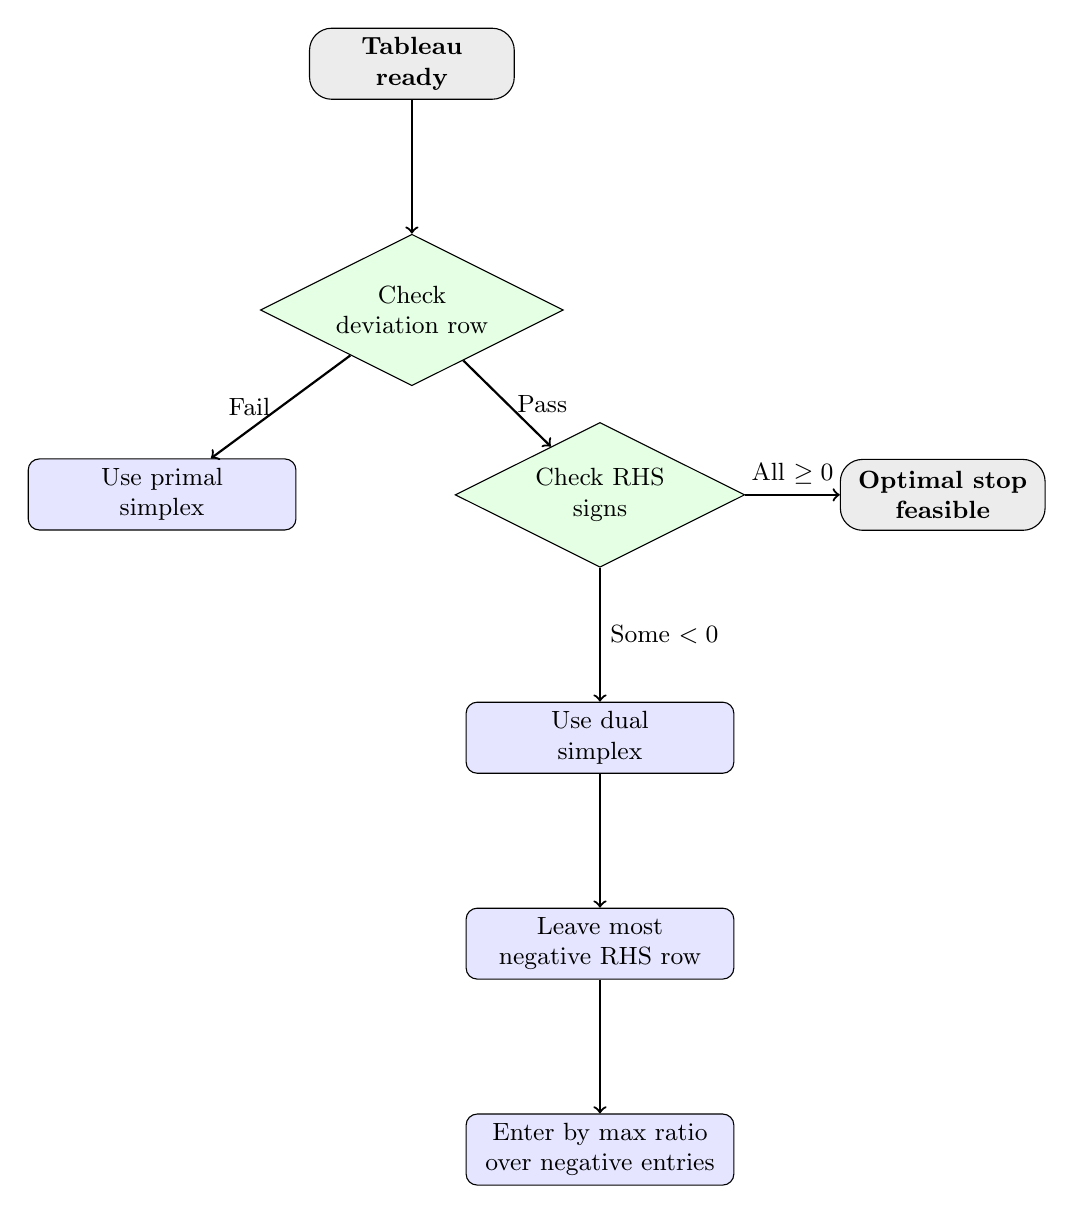
\begin{tikzpicture}[node distance=1.7cm]
\node (A) [term] {Tableau\\ready};
\node (B) [dec, below=of A] {Check\\deviation row};
\node (C) [proc, below left=1.4cm and 0.5cm of B] {Use primal\\simplex};
\node (D) [dec, below right=1.4cm and 0.5cm of B] {Check RHS\\signs};
\node (E) [term, right=1.2cm of D] {Optimal stop\\feasible};
\node (F) [proc, below=of D] {Use dual\\simplex};
\node (G) [proc, below=of F] {Leave most\\negative RHS row};
\node (H) [proc, below=of G] {Enter by max ratio\\over negative entries};
\draw [arr] (A) -- (B);
\draw [arr] (B) -- node [left, font=\small] {Fail} (C);
\draw [arr] (B) -- node [right, font=\small] {Pass} (D);
\draw [arr] (D) -- node [above, font=\small] {All $\geq 0$} (E);
\draw [arr] (D) -- node [right, font=\small] {Some $<0$} (F);
\draw [arr] (F) -- (G);
\draw [arr] (G) -- (H);
\end{tikzpicture}
\end{document}
